
The abstract of the original publication by Blankenbach \etal (1989) \cite{blbc89} reads:
\begin{center}
{\it 
We have carried out a comparison study for a set of benchmark problems 
which are relevant for convection in the Earth’s mantle. The cases comprise 
steady isoviscous convection, variable viscosity convection and time-dependent 
convection with internal heating. We compare Nusselt numbers, velocity, 
temperature, heat-flow , topography and geoid data. Among the applied codes 
are finite-difference, finite-element and spectral methods. In a synthesis 
we give best estimates of the ‘true’ solutions and ranges of uncertainty. We
recommend these data for the validation of convection codes in the future.
}
\end{center}

The temperature is fixed to zero on top and to $\Delta T$ at the bottom, 
with reflecting symmetry at the sidewalls (i.e. $\partial_x T=0$) 
and there are no internal heat sources. 
Free-slip conditions are implemented on all boundaries. 

The Rayleigh number is given by
\[
\Ranb = \frac{\alpha g_y \Delta T h^3 }{\kappa \nu}
=\frac{\alpha g_y \Delta T h^3 \rho^2 c_p}{k \mu}
\]
The initial temperature field is given by 
\[
T(x,y)=(1-y) - 0.01\cos(\pi x) \sin(\pi x)
\]
The perturbation in the initial temperature fields leads to 
a perturbation of the density field and sets the fluid in motion. 

Depending on the initial Rayleigh number, the system ultimately reaches a 
steady state after some time. 

\begin{center}
a)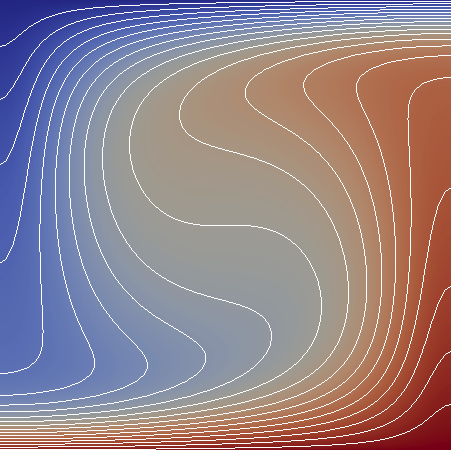
\includegraphics[width=4.5cm]{images/benchmark_blbc89/temp1a}
b)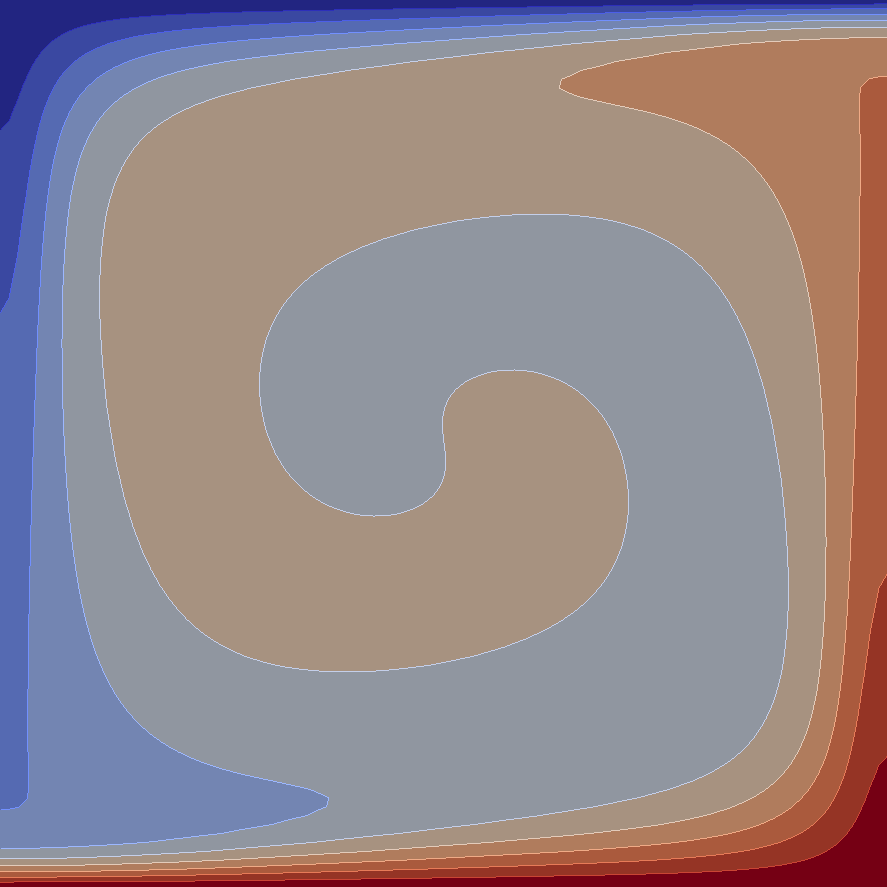
\includegraphics[width=4.5cm]{images/benchmark_blbc89/temp1b}
c)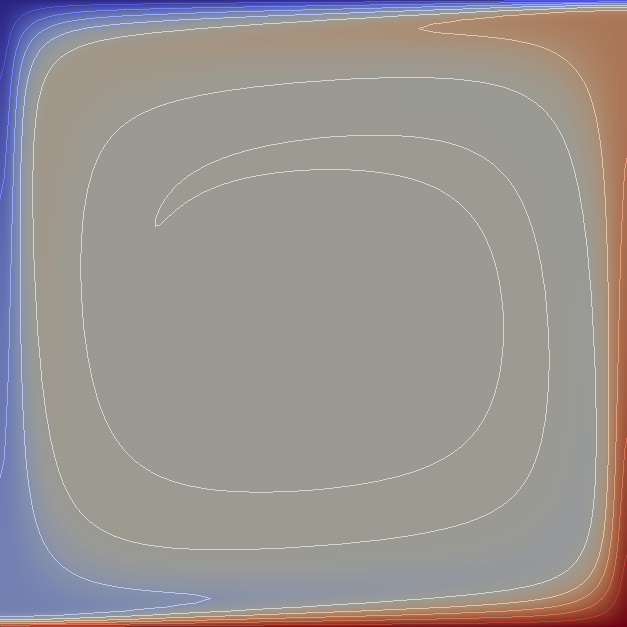
\includegraphics[width=4.5cm]{images/benchmark_blbc89/temp1c}\\
{\captionfont Temperature fields at steady-state for 
$\Ranb=10^4$ (a), $\Ranb=10^5$ (b), $\Ranb=10^6$ (c).
Obtained with \elefant code \cite{thie14}.}
\end{center}


\begin{center}
a)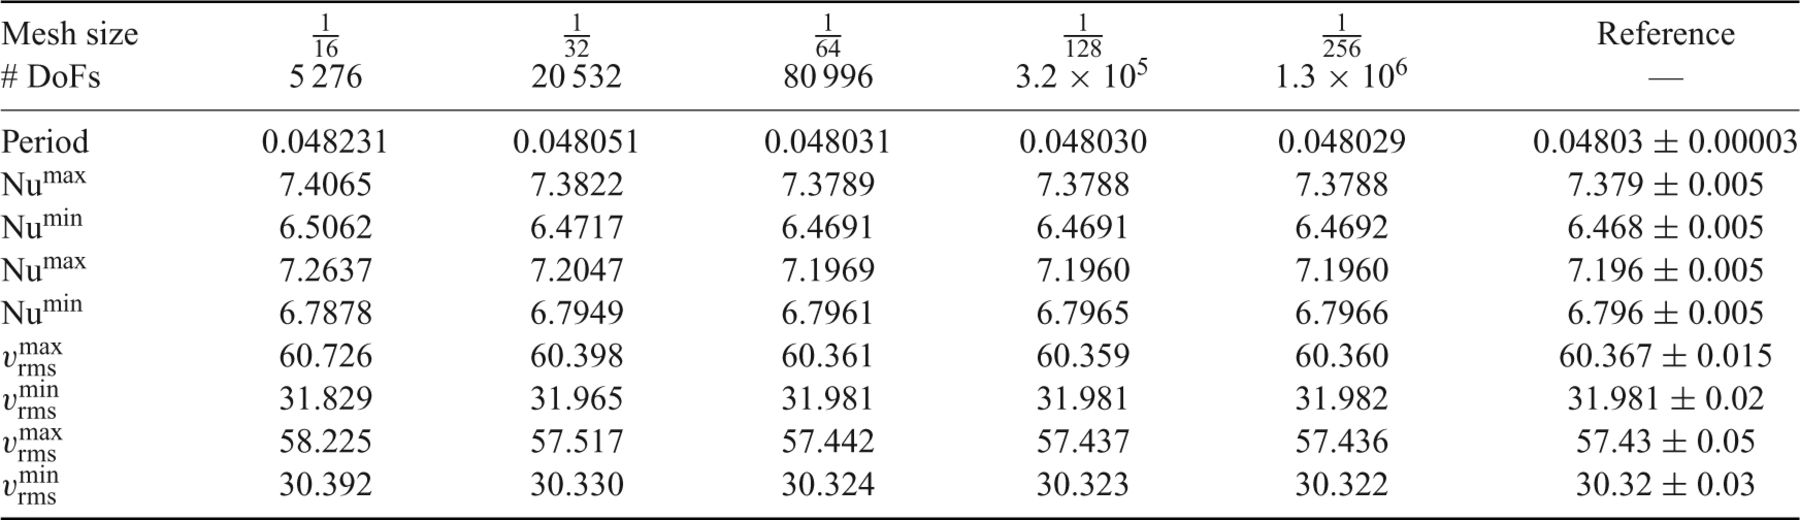
\includegraphics[width=13cm]{images/benchmark_blbc89/krhb12a}
b)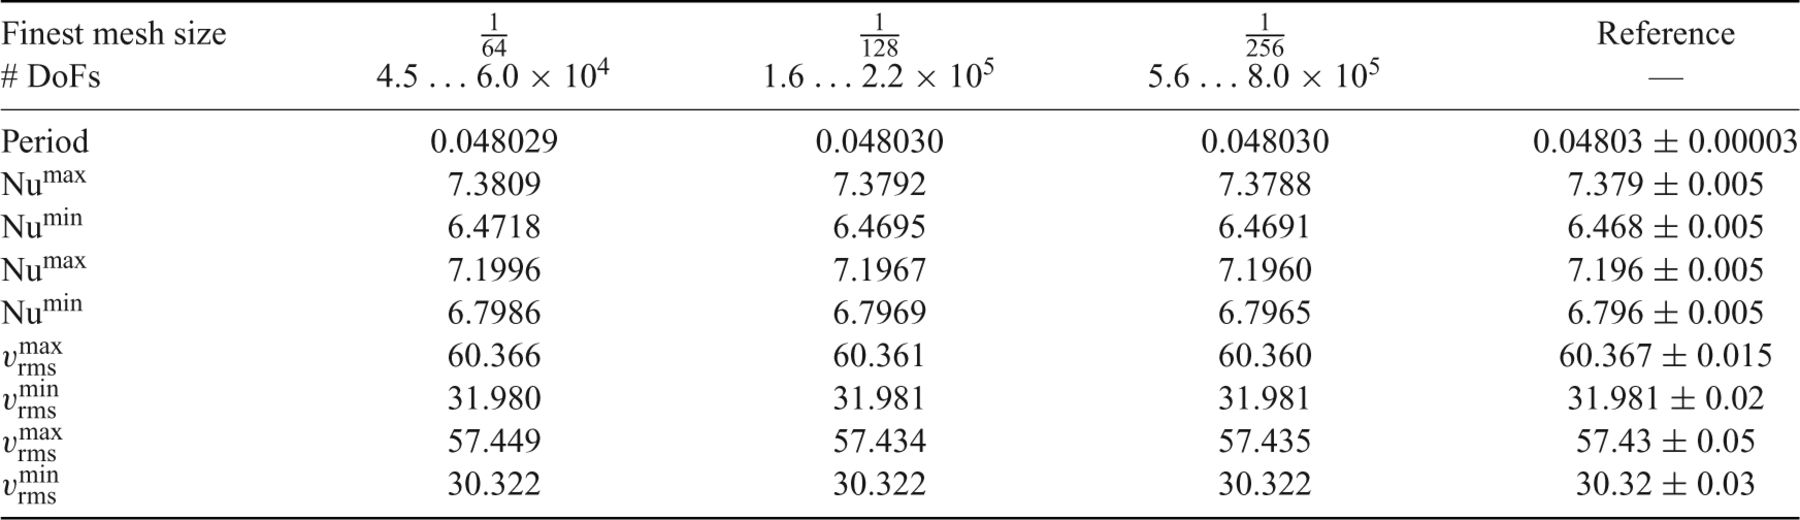
\includegraphics[width=13cm]{images/benchmark_blbc89/krhb12b}\\
{\captionfont 
a) Results for the 2-D benchmark problem with uniform mesh refinement. 
\# DoFs indicates the number of degrees of freedom.
Reference results from Blankenbach \etal (1989).
b) Results with adaptive mesh refinement. The number of degrees of freedom (\# DoFs) for
each finest mesh size $h$ varies between time steps; 
the indicated numbers provide a typical range.}
\end{center}


\begin{center}
\begin{tabular}{llcccc}
\hline
          &           & \cite{blbc89} &  \cite{tack94}  & \cite{king09}  & \elefant  \\
\hline
\hline
$\Ranb=10^4$ & $\upnu_{rms}$ &  $42.864947  \pm 0.000020$ & 42.775 (0.2\%) & 42.867  (0.005\%) & 42.867 (0.01\%) \\ 
             & $\Nunb$       &  $4.884409   \pm 0.000010$ & 4.878  (0.1\%) & 4.885   (0.02\%)  & 4.882  (0.05\%)\\
$\Ranb=10^5$ & $\upnu_{rms}$ &  $193.21454  \pm 0.00010 $ & 193.11 (0.05\%)& 193.248 (0.02\%)  & 193.255 (0.02\%)\\
             & $\Nunb$       &  $10.534095  \pm 0.000010$ & 10.531 (0.03\%)& 10.536  (0.02\%)  & 10.507 (0.26\%) \\
$\Ranb=10^6$ & $\upnu_{rms}$ &  $833.98977  \pm 0.00020 $ & 833.55 (0.05\%)& 834.353 (0.04\%)  & 834.712   (0.08\%)\\
             & $\Nunb$       &  $21.972465  \pm 0.000020$ & 21.998 (0.1\%)& 21.981  (0.04\%)  & 21.695  (1.2\%)\\
\hline
\end{tabular} \\
{\captionfont Steady state Nusselt number and Vrms measurements as reported in the literature and 
obtained with \elefant on a $200\times 200$ grid.}
\end{center} 


\Literature: Travis \etal (1990) \cite{trab90},
Ogawa (1993) \cite{ogaw93},
Trompert \& Hansen (1998) \cite{trha98},
Christon \etal (2002) \cite{chgs02},
Chiu-Webster \etal (2008) \cite{chhl08},
Kameyama \etal (2005) \cite{kaks05},
King (2009) \cite{king09},
Beuchert \& Podlachikov (2010) \cite{bepo10},
Leng \& Zhong (2011) \cite{lezh11},
Davies \etal (2011) \cite{dawk11},
Vynnytska \etal (2013) \cite{vyrc13},
\aspect{} manual \cite{aspectmanual},
Trim \etal (2021) \cite{trbs21},
\stone 3.



